% Compile: pdflatex paper_en.tex
\documentclass[10pt,twocolumn]{article}
\usepackage[a4paper,margin=18mm]{geometry}
\usepackage{graphicx}
\usepackage{amsmath}
\usepackage{amssymb}
\usepackage{booktabs}
\usepackage{enumitem}
\usepackage[hidelinks]{hyperref}

\setlength{\columnsep}{6mm}

\begin{document}

\twocolumn[{%
  \begin{center}
    {\LARGE\bfseries LoRA Fine-Tuning of a Personally-Created Character for Image Generation}\\
    \vspace{0.6em}
    {\large An Empirical Study under Few-Shot Conditions on a Consumer-Grade GPU}\\
    \vspace{1.2em}
    {\large Masato Suzuki (Masafy)}\\
    \vspace{0.4em}
    {May 22, 2026}
  \end{center}
  \vspace{1.0em}
  {\centering\textbf{Abstract}\par}
  \vspace{0.4em}
  \begingroup\small
  \noindent This report describes fine-tuning of the latent diffusion model Stable Diffusion 1.5 via Low-Rank Adaptation (LoRA), for the purpose of generating novel illustrations of an original character, ``Masafee'' --- a red-panda character created by the author and published as a messaging-app sticker set. No paid cloud computing resources were used; all training was performed on a single consumer-grade NVIDIA GeForce RTX 3060 (12\,GB VRAM) installed in the author's home PC. From an existing set of 16 stickers, 13 were selected by quality criteria as the training set. Three experiments were conducted: (1) an initial training run to verify feasibility, (2) a six-condition comparison varying the base model, learning rate, and LoRA rank, and (3) an ablation over training epochs from 10 to 60. We show experimentally that (a) the choice of base model has the largest impact on output quality, with an illustration-oriented base resolving background and style mismatches; (b) training performance reaches a plateau at roughly 30 epochs, beyond which there is no improvement and mild overfitting appears; and (c) the effective upper bound on output quality is governed by the number of training images. The study demonstrates that fine-tuning a personally-owned character can be completed practically on a single consumer-grade GPU, without paid cloud resources.

  \par\medskip
  \noindent\textbf{Keywords:}\ image generation, latent diffusion model, Stable Diffusion, low-rank adaptation, LoRA, fine-tuning, character generation, consumer-grade GPU
  \endgroup
  \vspace{2.0em}
}]

\section{Introduction}
Text-to-image diffusion models have advanced rapidly, and open-weight models such as Stable Diffusion are now usable at the individual level. Pre-trained on vast and diverse image corpora, these models possess general-purpose generation ability. However, consistently generating a \emph{specific} original character not present in the pre-training distribution, while preserving its identity, is fundamentally difficult with a general-purpose model alone: the mode corresponding to that character is absent, or of extremely low density, in the pre-training distribution. Additional fine-tuning is therefore required to make the model acquire the target concept.

Naive fine-tuning that updates all parameters faces two problems: (i) the computational and memory cost of updating billions of parameters, and (ii) catastrophic forgetting and overfitting under scarce data. Low-Rank Adaptation (LoRA) mitigates both by freezing the pre-trained weights and learning only low-rank difference matrices, enabling injection of a specific concept with modest compute and few training images.

The motivation of this work is practical and concrete. The author created an original red-panda character, ``Masafee,'' published as a messaging-app sticker set (16 stickers). The starting point is the desire to generate unrecorded poses and scenes of this character without additional hand-drawing. While paid cloud computing (e.g., Google Colab Pro+) was initially considered, this study verifies whether the entire workflow can be completed using only a single consumer-grade GPU available at home. The specific research questions are:
\begin{itemize}[leftmargin=2.4em,topsep=2pt,itemsep=1pt]
  \item[\textbf{Q1.}] Can novel poses be generated with preserved character identity from $\sim$13 few-shot reference images?
  \item[\textbf{Q2.}] What factor is rate-limiting for output quality (base model, learning rate, LoRA rank, or epoch count)?
  \item[\textbf{Q3.}] Does increasing the number of training epochs improve quality monotonically?
\end{itemize}
The contribution of this paper is to provide experimental answers to these questions, together with a reproducible procedure.

\section{Preliminaries}
This section gives the formulation of diffusion models, latent diffusion models, and low-rank adaptation needed for the subsequent discussion.

\subsection{Diffusion Probabilistic Models}
A diffusion model is a latent-variable generative model consisting of a \emph{forward process} that gradually adds Gaussian noise to data, and a \emph{reverse process} that traces it back. For data $x_0\sim q(x_0)$, the forward process is a Markov chain with a variance schedule $\{\beta_t\}_{t=1}^{T}$ ($0<\beta_t<1$):
\begin{equation}
q(x_t\mid x_{t-1}) = \mathcal{N}\!\big(x_t;\,\sqrt{1-\beta_t}\,x_{t-1},\,\beta_t\mathbf{I}\big).
\end{equation}
Defining $\alpha_t:=1-\beta_t$ and $\bar\alpha_t:=\prod_{s=1}^{t}\alpha_s$, the reproductive property of the Gaussian yields a closed form for the state at any step $t$ directly from $x_0$:
\begin{equation}
x_t = \sqrt{\bar\alpha_t}\,x_0 + \sqrt{1-\bar\alpha_t}\,\epsilon,\qquad \epsilon\sim\mathcal{N}(0,\mathbf{I}).
\label{eq:closedform}
\end{equation}
As $t\to T$, $\bar\alpha_t\to 0$ and $x_T$ approaches a standard normal. The reverse process is represented by a noise-predicting network $\epsilon_\theta$ with parameters $\theta$, and training minimizes the noise-prediction loss (a simplified variational bound)
\begin{equation}
\mathcal{L}(\theta)=\mathbb{E}_{x_0,\,\epsilon,\,t}\Big[\,\big\lVert\epsilon-\epsilon_\theta(x_t,t,c)\big\rVert_2^2\,\Big],
\label{eq:loss}
\end{equation}
where $c$ is the conditioning variable, here the embedding of a text description. Equation~\eqref{eq:loss} is evaluated by sampling $t$ uniformly and constructing $x_t$ via Eq.~\eqref{eq:closedform}.

\subsection{Latent Diffusion Models and Architecture}
Running the diffusion process directly in pixel space is computationally inefficient. The latent diffusion model (LDM) adopted by Stable Diffusion compresses an image into a low-dimensional latent representation $z_0=\mathcal{E}(x_0)$ via the encoder $\mathcal{E}$ of a variational autoencoder (VAE), and runs the diffusion process in latent space. Generated latents are restored to pixel space by the decoder $\mathcal{D}$ ($\hat{x}=\mathcal{D}(z_0)$). The noise predictor $\epsilon_\theta$ uses a U-Net architecture, into which the text condition $c$ is injected at each resolution level through \emph{cross-attention}. The condition $c$ is the embedding sequence produced by a text encoder (the text tower of CLIP) mapping the input sentence to token embeddings. The SD~1.5 family targeted here is a representative open-weight model of this LDM design.

\subsection{Conditional Generation and Classifier-Free Guidance}
To strengthen adherence to the condition $c$, classifier-free guidance (CFG) is widely used at inference. Combining the conditional prediction $\epsilon_\theta(x_t,t,c)$ and the unconditional prediction $\epsilon_\theta(x_t,t,\varnothing)$ ($\varnothing$ being the empty condition), an extrapolated prediction is used with guidance scale $s\ge 1$:
\begin{equation}
\tilde\epsilon_\theta(x_t,t,c)=\epsilon_\theta(x_t,t,\varnothing)+s\big(\epsilon_\theta(x_t,t,c)-\epsilon_\theta(x_t,t,\varnothing)\big).
\end{equation}
In this study, $s$ (the implementation's \texttt{scale}) was set around $7$.

\subsection{Low-Rank Adaptation (LoRA)}
Let a weight matrix of a linear layer of the pre-trained model be $W_0\in\mathbb{R}^{d\times k}$. Whereas full fine-tuning updates $W_0$ itself, LoRA freezes it and learns only a low-rank difference. The adapted weight is written
\begin{equation}
W' = W_0 + \Delta W,\qquad \Delta W=\frac{\alpha}{r}\,B A,
\label{eq:lora}
\end{equation}
where $B\in\mathbb{R}^{d\times r}$, $A\in\mathbb{R}^{r\times k}$, and the rank $r$ satisfies $r\ll\min(d,k)$. The scalar $\alpha$ scales the adaptation, whose effective strength is proportional to $\alpha/r$. Only $A,B$ are trained; their parameter count $r(d+k)$ is far smaller than the $dk$ of full fine-tuning. By convention $A$ is Gaussian-initialized and $B$ is zero-initialized, guaranteeing $\Delta W=0$ at the start of training and a continuous departure from the pre-trained model. We apply LoRA to the attention and projection layers of the SD~1.5 U-Net and text encoder. We refer to $r$ in Eq.~\eqref{eq:lora} as the ``LoRA rank'' and $\alpha$ as ``alpha.''

\subsection{Terminology}
Table~\ref{tab:notation} summarizes key terms used in this paper.

\begin{table}[t]\centering\small
\caption{Key terminology}
\label{tab:notation}
\begin{tabular}{ll}
\toprule
Term & Description \\
\midrule
EMA & Exponential moving average; a smoothed \\
    & copy of weights, stored by \texttt{emaonly}. \\
Bucketing & Grouping images of differing aspect \\
          & ratios into resolution buckets. \\
Gradient & Recomputing intermediate activations \\
checkpointing & to reduce VRAM usage. \\
Mixed precision & Using bf16 etc. for speed and memory. \\
SDPA & PyTorch's native fast attention kernel. \\
Trigger word & A unique token bound to the concept. \\
\bottomrule
\end{tabular}
\end{table}

\section{Problem Formulation}
Let the target character be $\mathcal{C}$ and its set of reference images be $\mathcal{X}=\{x^{(1)},\dots,x^{(N)}\}$ (here $N=13$). Each image $x^{(i)}$ is given a caption $c^{(i)}$ containing a unique trigger word $\tau$ (here \texttt{masafee}). The goal is to learn a LoRA difference $\Delta\theta$ (the collection of $\{A,B\}$ in Eq.~\eqref{eq:lora}), while keeping the pre-trained noise predictor $\epsilon_\theta$ frozen, so that images preserving the identity of $\mathcal{C}$ can be generated from any prompt $p$ containing $\tau$. Training is formulated as minimizing the loss of Eq.~\eqref{eq:loss} over $\mathcal{X}$:
\begin{equation}
\Delta\theta^{\star}=\arg\min_{\Delta\theta}\ \mathbb{E}_{i,\,\epsilon,\,t}\Big[\big\lVert\epsilon-\epsilon_{\theta+\Delta\theta}(z_t^{(i)},t,c^{(i)})\big\rVert_2^2\Big],
\end{equation}
where $z_t^{(i)}$ is the latent obtained by applying Eq.~\eqref{eq:closedform} to $\mathcal{E}(x^{(i)})$. Since $N$ is small, the problem is essentially few-shot, and both the expressiveness of $\Delta\theta$ (governed by $r$) and the amount of training (epoch count) are rate-limiting for output quality through the generalization--overfitting trade-off.

\section{Method}
\subsection{Computing Environment}
The computing environment is shown in Table~\ref{tab:env}. Because the training toolchain could not resolve its dependencies on the OS-default Python 3.14, an isolated Python 3.11 environment was built with the lightweight manager \texttt{uv}. This is a practical consideration when building a machine-learning environment on a bleeding-edge distribution.

\begin{table*}[t]\centering\small
\caption{Computing environment}
\label{tab:env}
\begin{tabular}{ll}
\toprule
Item & Detail \\
\midrule
GPU & NVIDIA GeForce RTX 3060 (12\,GB VRAM, Ampere, compute capability 8.6) \\
CPU / RAM & 20 logical cores / 30\,GB \\
OS & Ubuntu 26.04 LTS \\
Framework & kohya-ss/sd-scripts, PyTorch 2.5.1 + CUDA 12.4 \\
Python & Python 3.11 provisioned separately via \texttt{uv} (system Python 3.14 incompatible) \\
\bottomrule
\end{tabular}
\end{table*}

\subsection{Training Data and Selection Criteria}
The training data was drawn from the author-created sticker set ``Masafee'' (16 stickers). As shown in Figure~\ref{fig:data}, the character is based on a red panda and has temporally consistent identifying features: goggles, a crown-patterned bandana, and a ringed tail. From the 16, we excluded (i) one image of severely low resolution that degrades under resampling, and (ii) two rough sketches whose line style deviates from the rest and harms style consistency, yielding the training set $\mathcal{X}$ of \textbf{13 images}. All selected images are $1000\times1000$~px RGB; the composition breakdown is 8 face close-ups, 3 full-body, 1 upper-body, and 1 distinct scene.

\begin{figure*}[t]\centering

\includegraphics[width=0.95\textwidth]{figures/fig1_trainingdata.png}
\caption{The 13 Masafee stickers constituting the training set $\mathcal{X}$.}
\label{fig:data}
\end{figure*}

\subsection{Caption Design and Trigger-Word Binding}
Each caption $c^{(i)}$ was designed from the viewpoint of concept binding. The trigger word $\tau=\texttt{masafee}$ was fixed at the start of every caption, and \emph{attributes intended to be variable} (pose, expression, background, presence of text) were enumerated explicitly as tags. Explicitly stated attributes are learned as independent concepts and become controllable at inference. Conversely, \emph{invariant character features} (goggles, bandana, etc.) were deliberately left undescribed, so that their visual features are residually bound to $\tau$. This exploits the empirical rule that visual regularities absent from captions are absorbed into the trigger word. Text baked into the stickers was handled by noting ``with text'' in captions rather than cropping, so that text and the character body are learned as separate factors.

\subsection{Training Configuration}
The optimizer was 8-bit AdamW, quantizing the optimizer state to reduce VRAM consumption. Mixed precision used bfloat16, and attention used PyTorch's native SDPA, avoiding a dependency on additional libraries. Gradient checkpointing and aspect-ratio bucketing were also employed, and horizontal flip was applied as data augmentation. The number of optimization steps per epoch is $\lceil N\cdot R/B\rceil$ ($R$: image repeats, $B$: batch size).

\section{Experiments}
The study comprises three experiments.

\textbf{Experiment 1 (Feasibility):} Initial training used standard SD~1.5 (\texttt{v1-5-pruned-emaonly}), $512$~px resolution, LoRA rank $r=32$ / $\alpha=16$, learning rate $1\!\times\!10^{-4}$, batch size 2, for 16 epochs (1040 steps).

\textbf{Experiment 2 (Factor sweep):} To isolate the rate-limiting factor of output quality, six conditions were trained and compared at $768$~px, 30 epochs each, varying base model $\in\{$standard SD1.5, Counterfeit-V3.0$\}$, learning rate $\in\{1\!\times\!10^{-4}, 2\!\times\!10^{-4}\}$, and LoRA rank $\in\{16,32\}$. Weights were saved at epochs 10/20/30 and evaluated with five prompts absent from the training set, forming comparison grids.

\textbf{Experiment 3 (Epoch ablation):} The best condition from Experiment~2 was extended to 60 epochs, comparing outputs at epochs 30/40/50/60. With a fixed random seed, results up to epoch 30 reproduce Experiment~2 identically, adding epochs 40--60.

\section{Results}
\subsection{Experiment 1: Feasibility}
Initial training took about 9 minutes on the RTX 3060, using about 3\,GB of VRAM. In generation tests, the character's identifying features (goggles, bandana, facial markings) were reproduced well, and poses absent from the training set (jumping, sleeping, astronaut suit) were generated successfully. Thus \textbf{Q1 is confirmed affirmatively}. Two systematic weaknesses were observed: (i) backgrounds darkened even when ``white background'' was specified in the caption, and (ii) shading was applied more strongly than in the flat coloring of the originals.

\subsection{Experiment 2: Dominance of the Base Model}
The six-condition comparison (Figure~\ref{fig:sweep}) gave a clear result. All three standard-SD1.5-base conditions exhibited background darkening and excessive shading, while all three Counterfeit-V3.0-base conditions produced clean white backgrounds and flat coloring close to the original sticker style. That is, the weaknesses of Experiment~1 were resolved \textbf{not by tuning the learning rate or LoRA rank, but by switching the base model to an illustration-oriented one}. Differences attributable to learning rate and LoRA rank were small compared to those between base models. Hence \textbf{for Q2 we conclude that, among the factors examined, the base model choice is dominant}. This is theoretically consistent with the structure of Eq.~\eqref{eq:lora}: since LoRA learns only a \emph{difference} from the pre-trained model, the stylistic prior of the output is strongly governed by the base model. The best condition was Counterfeit + learning rate $1\!\times\!10^{-4}$ + LoRA rank 32 (hereafter cf\_lr1\_d32).

\begin{figure*}[t]\centering
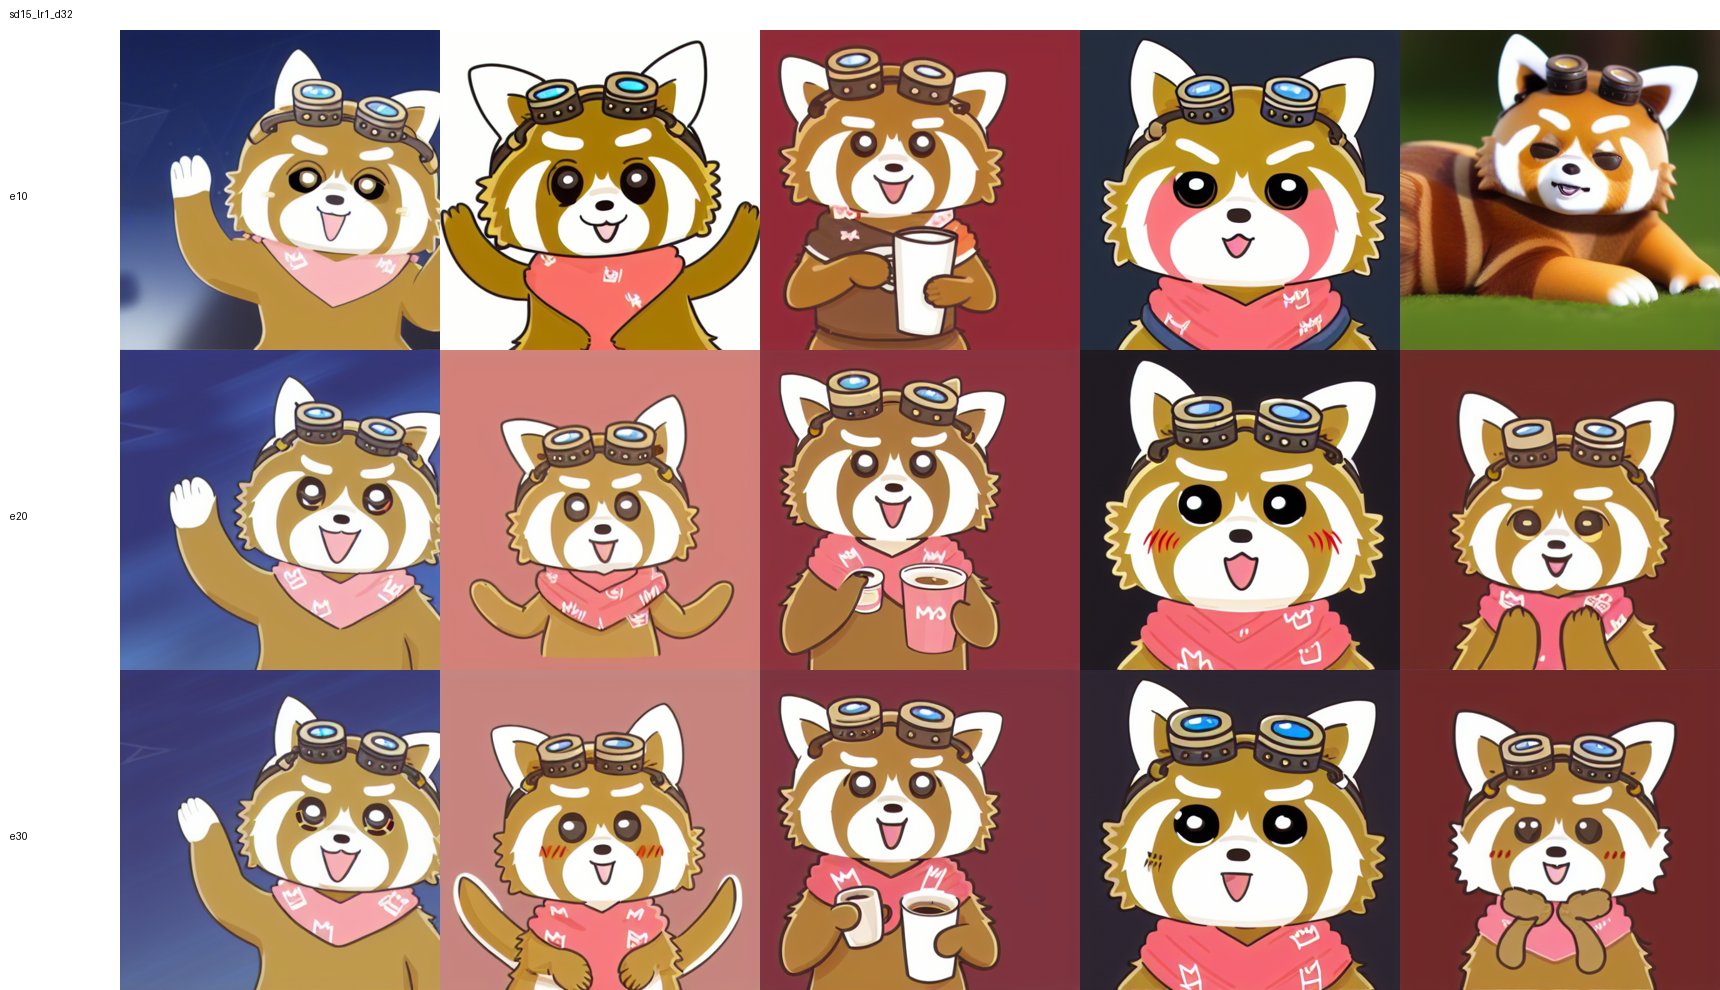
\includegraphics[width=0.78\textwidth]{figures/fig2a_sd15.png}\\[6pt]
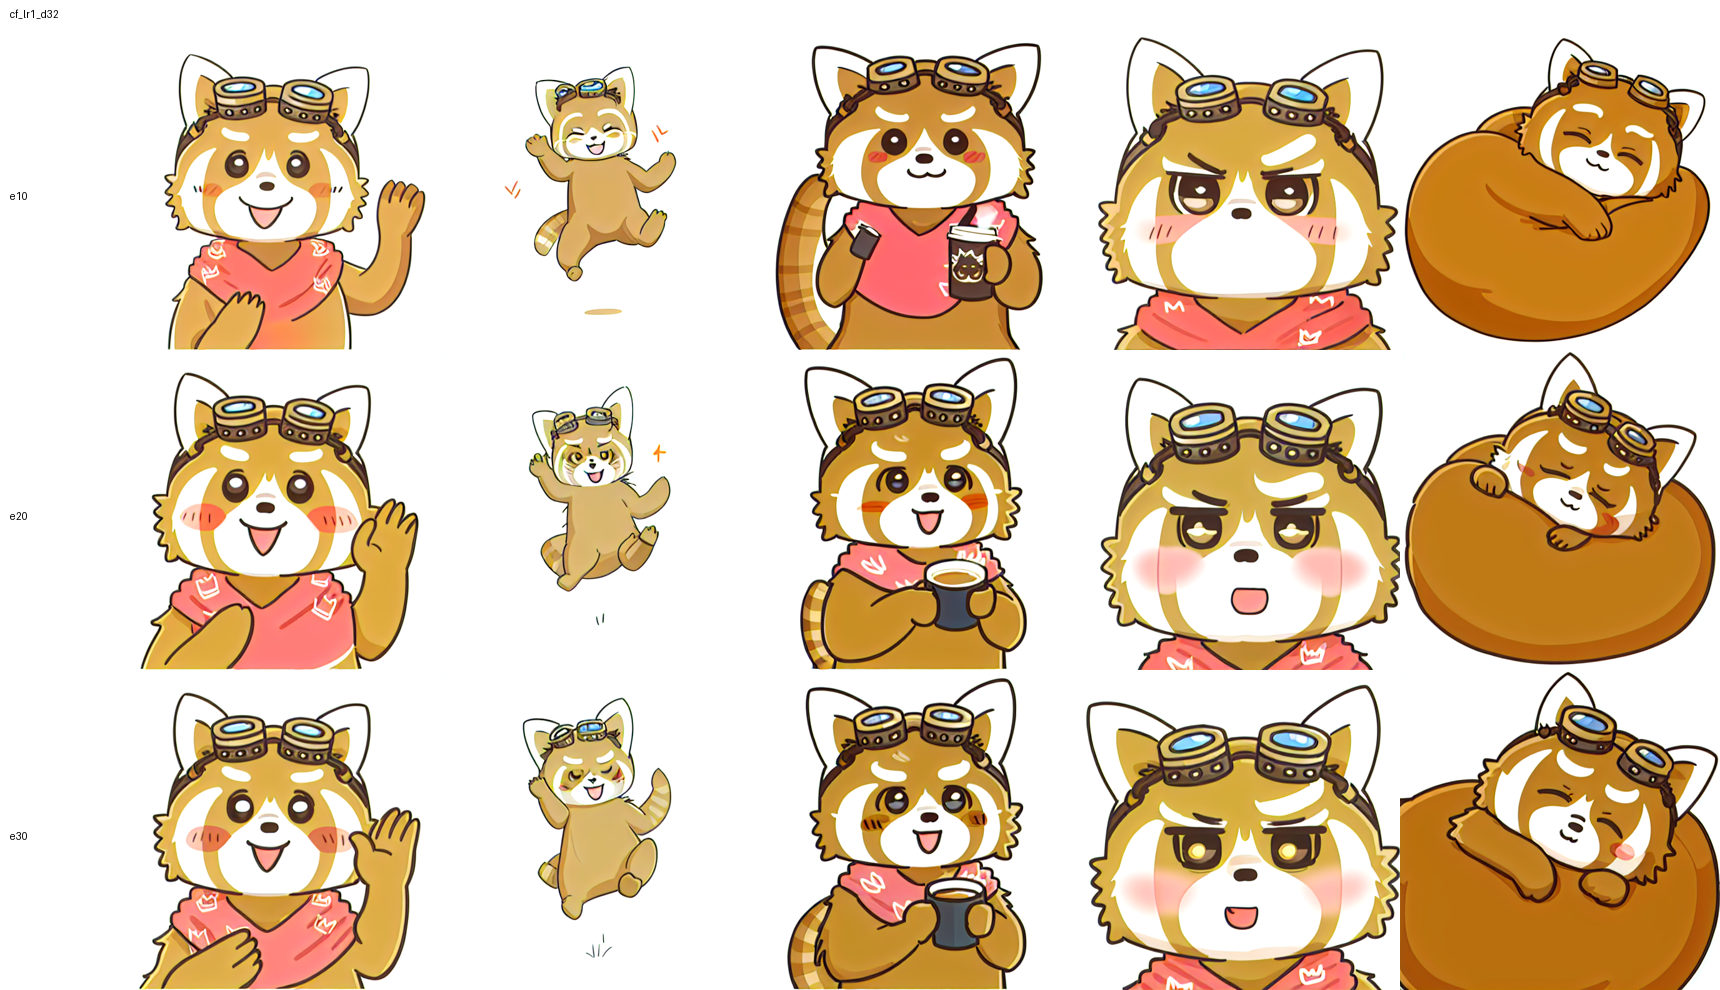
\includegraphics[width=0.78\textwidth]{figures/fig2b_counterfeit.png}
\caption{Representative sweep comparison. Top: standard SD~1.5 base. Bottom: Counterfeit base. Rows are epochs (10/20/30); columns are evaluation prompts.}
\label{fig:sweep}
\end{figure*}

\subsection{Experiment 3: Performance Plateau over Epochs}
Extending the best condition to 60 epochs (Figure~\ref{fig:epoch}), outputs at epochs 30/40/50/60 were visually nearly indistinguishable; \textbf{performance had already plateaued by epoch 30}. Moreover, at epochs 50--60 an increase in saturation was observed, interpreted as a mild sign of overfitting (memorization) to the training set. Hence \textbf{for Q3 we conclude that, under this data and configuration, increasing the epoch count beyond about 30 does not improve quality}. Under few-shot conditions, increasing epochs does not improve generalization but moves the system toward the overfitting side of the generalization--overfitting trade-off.

\begin{figure*}[t]\centering
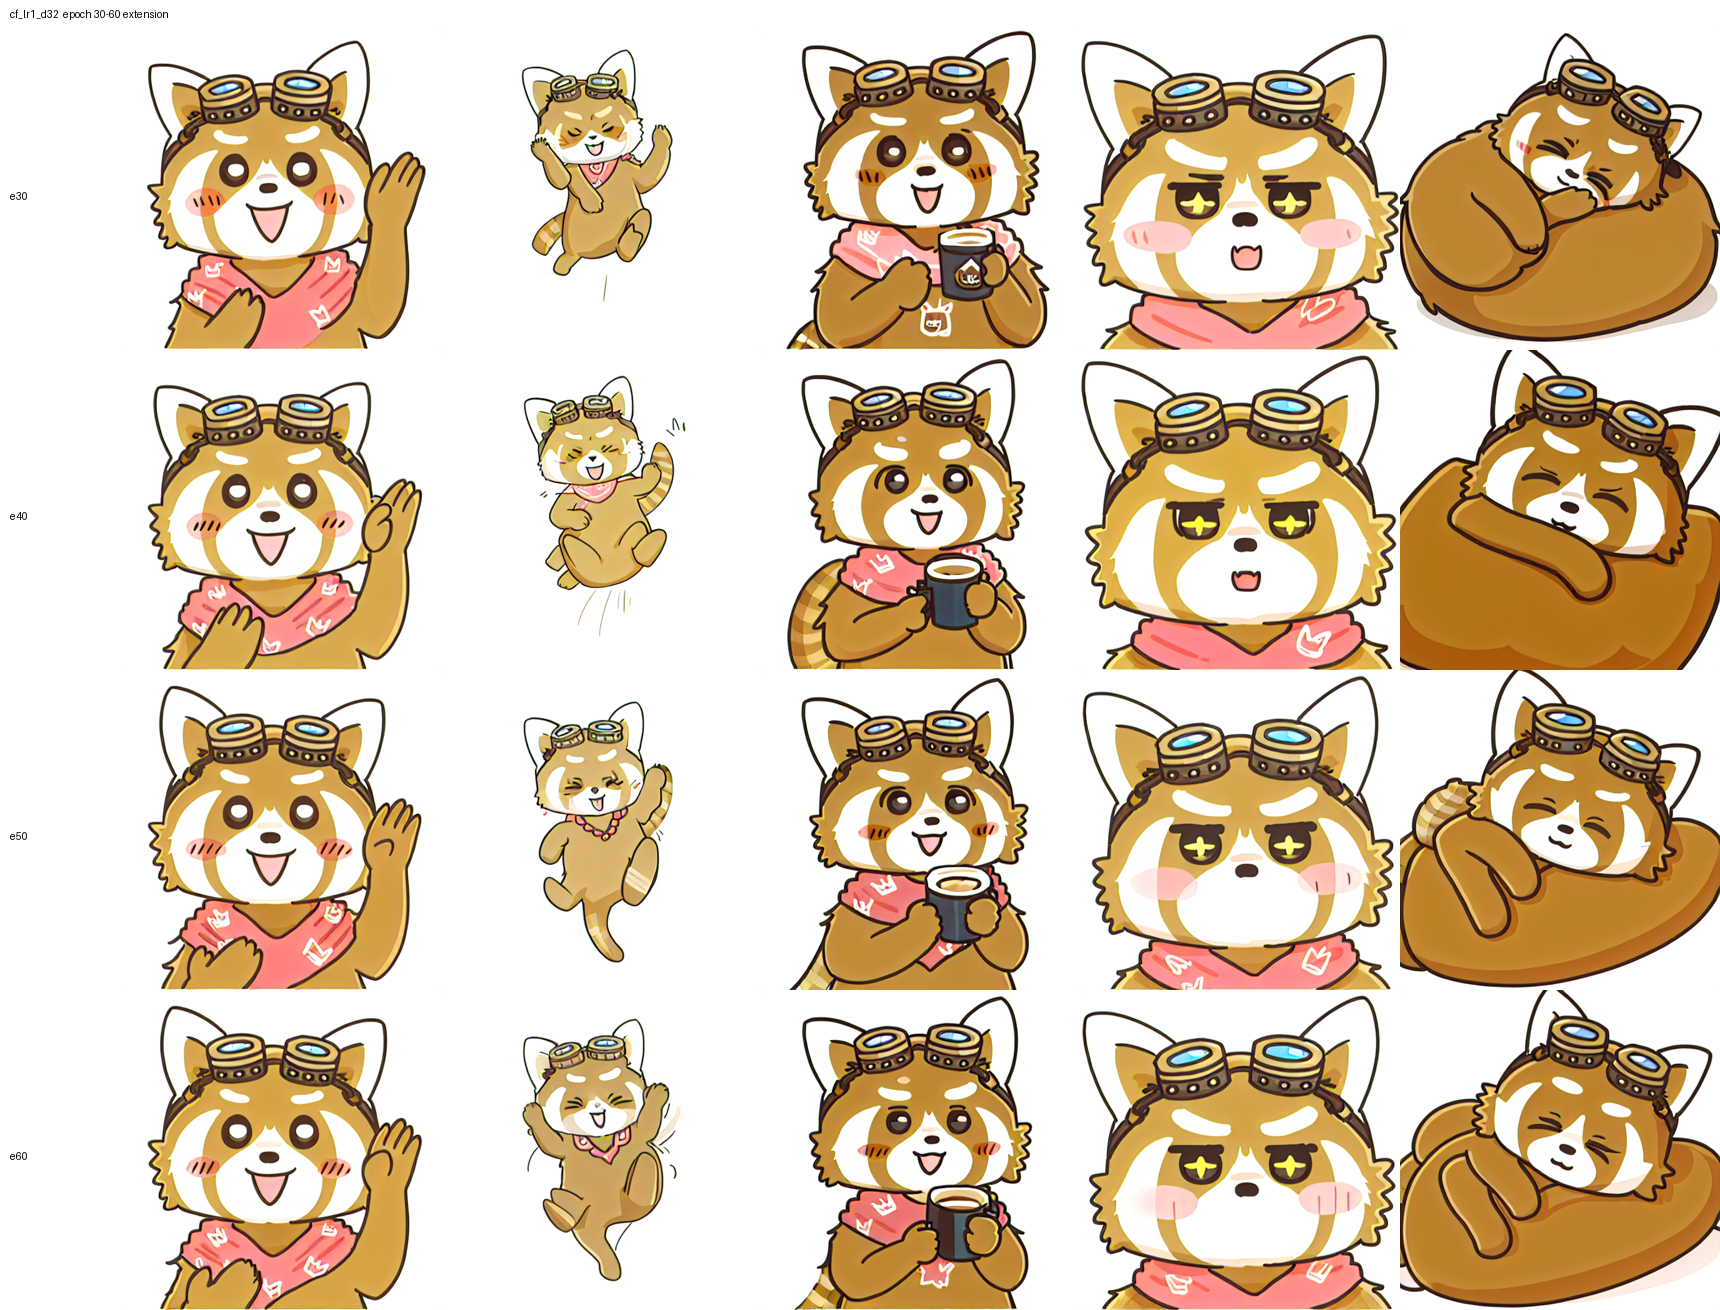
\includegraphics[width=0.78\textwidth]{figures/fig3_epoch.png}
\caption{cf\_lr1\_d32 compared at epochs 30/40/50/60. Differences between rows are slight.}
\label{fig:epoch}
\end{figure*}

\subsection{Generation with the Final Model}
Using the best model (cf\_lr1\_d32, epoch 30), 12 scenes absent from the training set (dancing, having coffee, reading, playing an instrument, cooking, walking in the rain, etc.) were generated (Figure~\ref{fig:showcase}). All preserved character identity and the flat art style at a quality sufficient for practical use. In the rain scene, the background was initially overly dark and gloomy, attributable to the prompt not specifying background luminance; specifying ``bright, soft colors, light blue background'' explicitly and adding ``dark, scary'' to the negative prompt resolved it. This is a practical lesson that scene-dependent attributes should be conditioned explicitly.

\begin{figure*}[t]\centering

\includegraphics[width=0.82\textwidth]{figures/fig4_showcase.png}
\caption{Twelve novel poses generated by the best model.}
\label{fig:showcase}
\end{figure*}

\section{Discussion}
\textbf{Dominance of the base model and its implications.} The central finding is that output quality strongly depends on the choice of base model. As Eq.~\eqref{eq:lora} shows, LoRA learns only $\Delta W$, while the stylistic prior underlying generation is retained in the frozen $W_0$. When the target style (flat illustration) diverges from the prior (photorealism), a finite-rank $\Delta W$ cannot fully overwrite the style, leaving mismatches in background and shading. Selecting a base model consistent with the target style is therefore a design decision that precedes hyperparameter tuning.

\textbf{Overfitting and epoch count.} With as few as 13 images, once the total number of optimization steps exceeds a threshold, $\Delta\theta$ begins to memorize idiosyncratic configurations of the training set (background, palette, composition). Experiment~3 showed experimentally that the onset of this overfitting lies near epoch 30. The intuition that ``longer training improves results'' is incorrect under few-shot conditions; an appropriate epoch count exists, depending on data size.

\textbf{Quality ceiling set by data size.} Since the epoch count plateaus, the principal remaining degree of freedom for further quality gains is the addition of training images. The sample size $N=13$ itself sets the effective upper bound on attainable generalization performance.

\textbf{Sufficiency of consumer-grade GPUs.} Each training trial took 9--40 minutes on the RTX 3060, with VRAM usage of 3--8\,GB. For creating an SD1.5-scale character LoRA, paid cloud computing is not required; the workflow, including iterative experimentation, can be completed on a single consumer-grade GPU.

\section{Limitations and Future Work}
This study has the following limitations. First, evaluation is qualitative, based on visual inspection of comparison grids, without quantitative metrics such as CLIP similarity or Fréchet Inception Distance (FID). Second, the training set is a single character of 13 images, constraining the generalizability of the conclusions. Third, baked-in text was handled by caption description, without a controlled comparison against cropping. Fourth, each sweep condition was evaluated with a single seed, not capturing seed-induced variance. Future work includes expanding the training images, introducing quantitative metrics, validation with newer base models such as SDXL, and generalization to multiple characters.

\section{Conclusion}
Using only a consumer-grade GPU (RTX 3060), we performed LoRA fine-tuning for image generation of the author's original character ``Masafee.'' We showed experimentally, with a reproducible procedure, that novel-pose generation with preserved identity is possible from 13 few-shot reference images (Q1); that output quality depends most strongly, among the factors examined, on the choice of base model (Q2); and that training performance plateaus at about 30 epochs, beyond which further training does not improve quality (Q3). This study demonstrates that fine-tuning a personally-owned character can be completed practically on a single consumer-grade GPU, without paid cloud resources.

\appendix
\section{Key Hyperparameters (cf\_lr1\_d32)}
Base model: Counterfeit-V3.0 (SD1.5-family illustration model); resolution: $768\times768$; LoRA rank $r$ / $\alpha$: 32 / 16; learning rate: $1\!\times\!10^{-4}$ (cosine decay); optimizer: 8-bit AdamW; batch size: 2; epochs: 30 (recommended, $\sim$1950 steps); mixed precision: bfloat16; augmentation: horizontal flip; attention: SDPA.

\section{Reproducibility}
The full training environment, sweep results, epoch-extension artifacts, this paper, and all scripts are included in the public repository.

\end{document}
